\chapter{Results \& Evaluation} \label{Evaluation}

This chapter covers the evaluation of the developed payloads and defence mechanisms. 


\section{Payloads}

It is difficult to find an objective, quantitative measure of the effectiveness of a payload. It is influenced by too many outside factors and the specific context it is deployed in. However, it is possible to qualitatively evaluate whether or not it can reach its own specific goal, discounting any factors of the bigger picture of the attack, such as whether the information was useful or the success of planting the hardware. This section will discuss whether the payloads introduced in chapter \ref{Methodology} achieve their declared goal. Within this aspect, there can be a distinction between reliability and speed. Both of these factors are heavily influenced by the circumstances surrounding the attacked host. Speed specifically may have to be adjusted to the computational power of the target and reliability depends heavily on how well this speed is chosen. Too little wait jeopardizes the entire attack, and long delays may produce overhead. However, the more time overhead the more reliable the payload in different situations, since it will work on more and older computers. Reliability can also be impacted by the other processes running on the computer, such as Bad USB-specific defences, antivirus software, Updates etc. . To be able to make some claims as to the flexibility (and thereby reliability) of these attacks, this evaluation will be carried out on multiple devices, specifically including computers in which the payloads have never been executed before. The following computers were used;

\begin{itemize}
    \item Microsoft Surface Laptop 4, Processor: 11th Gen Intel(R) Core(TM) i7-1185G7 @3.00GHz, 16.0 GB installed RAM running Windows 11 Home version 23H2 (Used for payload development), without any additional Antivirus or Bad USB protection
    \item MSI Stealth 16 Studio A13V, Processor: 13th Gen Intel(R) Core(TM) i7-13700H @2.40 GHz, 32 GB installed RAM running Windows11 Home version 23H2, without any additional antivirus or BAD USB protection.
    \item family home computer
    \item silvan?
\end{itemize}
    
In the following, this section will go through all the payloads and describe their execution on the above-mentioned devices. For every evaluation, the computers were unlocked, connected to the internet, and Bluetooth turned off. All running applications and background processes, including Teams, Outlook, Vanguard, Spotify, etc., were closed unless otherwise mentioned. Every target device's keyboard layout was set to Swiss ISO. The payloads were manually executed through a separate device. 

\subsubsection{Register Email Forwarding}

GOAL: Enable Email forwarding to a desired Email address as an attempt to gather intelligence and eavesdrop on conversations. \\
PREREQUISITES: The new Outlook version has to be installed on the target and the desired email must be logged in. Furthermore, the email for forwarding has to be configured in the payload. 

Already on the first execution of this payload on the MSI laptop a common problem appears; Outlook requires an update to operate. 

\begin{figure}[H]
    \centering
    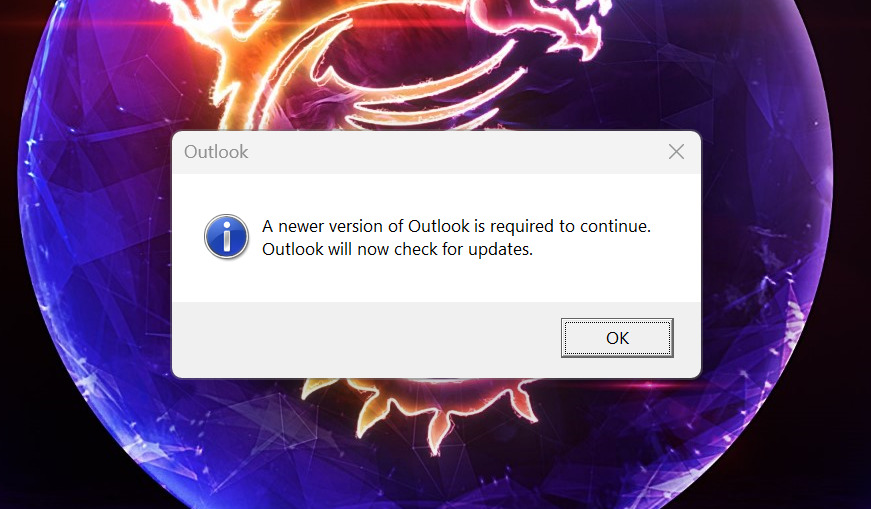
\includegraphics[width=0.5\linewidth]{visuals/outlook_requires_update.jpeg}
    \caption{Error Message after executing Forwarding Payload on MSI laptop}
    \label{fig:builtInTeensy}
    \cite{farhiMalboardNovelUser2019}
\end{figure}


Another big challenge with this payload is its UI focus. It requires a lot of settings menu navigation which is very time-sensitive. Short delays are detrimental here. Even for the MSI laptop which has the most compute of the tested devices, an especially long delay for opening Outlook and a delay of around 300ms between every navigation step is necessary to ensure that every TAB and ARROW input is correctly placed. \\
On the Microsoft Surface laptop, the attack worked as expected, which can be attributed to the fact that it was built while continuously being tested on this device. For none of the other test objects did the payload work out of the box, each would require updates, new logins or even lack the new Outlook completely. 

The conclusion for this payload is that it is not versatile and indeed requires a rather specific set of circumstances to work. Its UI focus makes this even harder since delays have to be high to accommodate the long loading times of an application like Outlook. If it works correctly, however, the payload can be very powerful and useful for gathering intelligence. 


\subsubsection{Disable Windows Event Logging}

GOAL: Disable Windows Event logging to hide possible traces another attack might leave. \\
PREREQUISITES: Windows 11

This payload has two versions; UI and CLI-based approaches, as discussed in chapter \ref{Implementation}. For the UI-based version, the usual problems occur; loading times, pop-up problems, and unforeseen reactions by the host. However, since this time the payload navigates through Windows Settings panels and not Outlook, some more continuity and speed can be expected. There are no server calls to be made that influence loading times, instead the process should be more straightforward. 
The Command Line Version should be even more reliable. It contains fewer steps and therefore less margin for error. It is expected to run smoothly on all test subjects.

The first execution of the UI-based approach proved once again its flakiness; Disabling Widows event logging on the MSI laptop would have also stopped another process, which caused the pop-up to confirm the action. This was not foreseen by the payload and therefore interrupted the process to the point where it exited the settings panel by selecting 'cancel' instead of 'apply' thereby ruining its progress. A second execution successfully stopped Windows event logging, since the pop-up did not appear again. However, it failed to close the settings window, leaving a trail of the attack. The navigation on the other side, was more reliable than what could be observed with the email forwarding payload which is as expected. \\
What was unexpected were language setting problems. When testing the payload on the TODO gaming desktop, it ran into problems because the search did not yield Windows event logging, but instead 'Windows Defender Advanced'. The payload would have to be adjusted to find the German 'Windows-Ereignisprotokoll'. After this adjustment, however, the next problem occurred; since the User did not have administrator rights, the settings options were greyed out and the payload had no chance of succeeding. \\
The payload worked well on the Surface Laptop, as expected since it was developed on it.

The CLI approach yielded much better results succeeding on the first try on the MSI laptop. As well as working on the custom-built gaming computer after adjusting the payload to enter the administrator password. As expected it also worked well on the Microsoft Surface Laptop. This result solidifies the superiority of a command line approach as opposed to navigating user interfaces. 


Conclusively it can be said that this payload works very well when applying the CLI approach. The UI version can work as well but requires a lot of fine-tuning, administrator access, and English as the system language. 



\subsubsection{Extract SSH hashes}

GOAL:\\ Extract SSH hashes from default storage on a device and send them to a command and control (C\&C) server.
PREREQUISITES: Windows 11 and a running C\&C server, in this case, Dropbox. Administrator rights are required

Since this script is working with default Windows settings, there are not a lot of challenges to be expected. On the MSI laptop, it worked flawlessly after some adjustments on the delays for opening the terminal. Since administrator access is not given on the custom gaming computer, the payload had to be adjusted to include the administrator password. With this adjustment, it was able to run successfully. The best results were again on the Windows Surface Laptop, where it executed flawlessly. 


\subsubsection{Extract Private Key Files}

GOAL: Find files that have extensions commonly used for private key files and send them to a C\&C server. \\
PREREQUISITES: Knowledge about the file system

This payload needs an entry point, some path to a local folder from which it can search through the files. If this is chosen too generally there may be permission issues. The entry point also heavily influences the time this payload takes to execute since it determines how many files the loop has to go through. The longer the script takes to execute, the easier it is to spot. \\
Since this payload does not require admin privileges one challenging step of opening an admin terminal is eliminated. One unexpected factor for errors is the validity length of the Dropbox access token. It expires within 4 hours. This means that in between saving the payload to the cable and the execution not more than those few hours may elapse. It was not a problem to adjust the payload for manual testing, however, this eliminates a C\&C server like Dropbox for boot scripts with unknown execution times. \\

The payload generally worked well on the Microsoft Surface laptop; its file system is known and an adequate entry point could be chosen. The execution was a success on the MSI laptop and the custom desktop as well. These good results could be due to the fact that apart from starting PowerShell, there are no loading times that can throw off the execution of the payload. Even waiting for the loop to end was not a problem; although delays were not adjusted to the expected search time, PowerShell still recognized and executed the command after finishing the loop.



\subsubsection{Steal Web Session Cookies}

GOAL: Figure out the target's default browser, then steal the web session cookies. \\
PREREQUISITES: None

This payload is pretty straightforward. Nevertheless, challenges for its flexibility arise. Executing the payload on the Microsoft Surface device went expectedly well, however, upon execution on the MSI laptop an error message occurred. Although the default browser on both of these devices is set to Firefox, their versions differ. While the Surface laptop had a slightly older version ( 129.0.1) the MSI laptop ran on the newest release, 129.0.2. This is reflected in the path to their cookies file. The .2 version stores the cookies at '\\Mozilla\\Firefox\\Profiles\\dpsymep9.default-release\\cookies.sqlite'  while .1 stores them at 'Mozilla\\Firefox\\Profiles\\umva4gfp.default-release\\cookies.sqlite' . This unexpected little, but crucial detail, derailed the execution of the script on the MSI laptop. The Chrome cookies path seems to be more robust; it worked without adjustments after changing the default for the MSI laptop to Chrome. The same problem occurred with the execution on the custom-built computer; it is running Firefox version wkbzpjnx. A more flexible version of this payload would check for versions and insert them as variables in the string, similar to how it does it with the Username environment variable. 

Apart from the version issues this payload performed well and as expected. 


\subsubsection{Iteratively End Processes}



GOAL: Certain processes should be ended as soon as they are detected as running. In whitelist mode, all programs except a few should be ended when they are detected as running.\\
PREREQUISITES: Windows 11, no admin rights required


This payload worked surprisingly well on the very first try. The MSI laptop posed no problem at all, not even delay adjustments had to be made. It worked as expected, terminating processes from the whitelist. As expected, the payload executed well on the Microsoft Surface, and on the desktop as well. \\
The only aspect that posed some problems was the minimizing of the window after the execution of the payload. It seemed that the 'ALT SPACE' keypresses were not registered by the device and were not acted upon. On every device, the window was simply left open creating an obvious drawback for this payload; it is easy to spot and stop manually. 

\subsubsection{Schedule Processes}

GOAL: Schedule a job on the target device to execute a chosen script at a chosen time. \\
PREREQUISITES: Windows, administrator privileges

In order to test this payload, I set the script of the job to be \verb|Get-Process|. Execution on the MSI laptop worked well. However, it is important to note, that executing the payload twice back to back will generate an error because the process 'ProcessJob' is already registered. To confirm the registration of the job, the Windows Scheduler Application can be used. The process should be listed under task scheduler library -> Microsoft -> Windows -> PowerShell -> ScheduledJobs. \\
Execution on the Surface Laptop went without issues as well. A challenge for the desktop is that the payload requires admin privileges. After adjusting the payload to enter the admin password, the payload is executed without any issues. 

\begin{figure}[H]
    \centering
    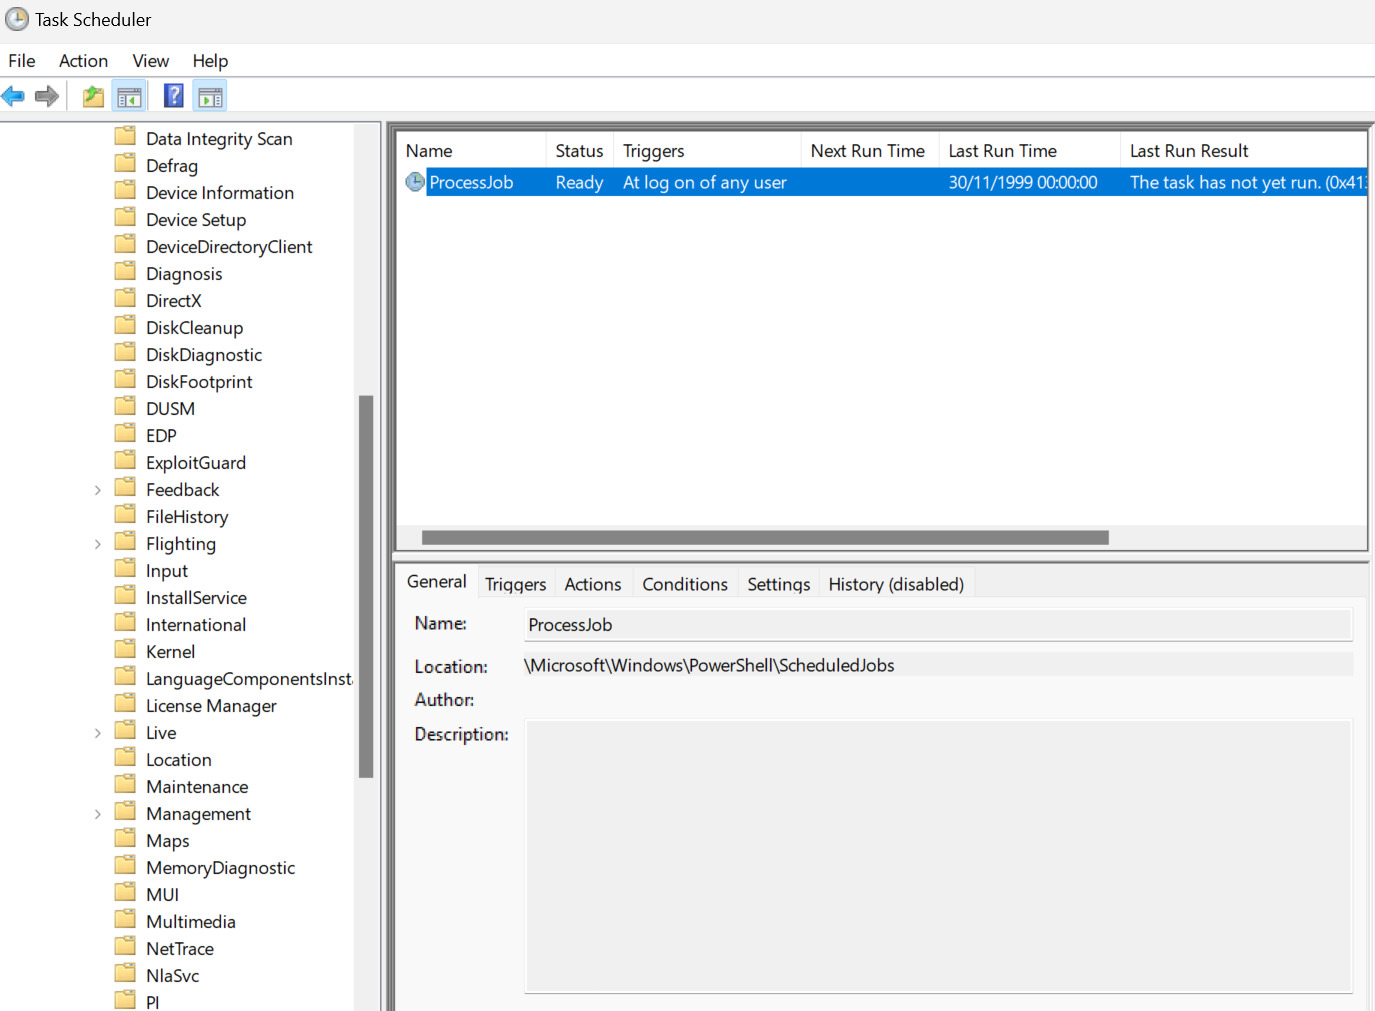
\includegraphics[width=0.5\linewidth]{visuals/task_scheduler_MSI.jpeg}
    \caption{Task Scheduler on the MSI laptop after successful registration of the Job}
    \label{fig:TaskScheduler}
\end{figure}




\subsection{Specific Usecases}

gaming
through a hub



\section{Defence}



This section will evaluate the speed and reliablility of the detection script.
It will evaluate the two components seperately; first it will take a look at the enumeration pattern detection and subsequently it will deal with the rate limiter.


\subsection{Enumeration Pattern Detection}

This subsection will describe an analysis of frames in order to evaluate the speed of the enumeration pattern detection. Since USB communication happens at very high speeds, it is impossible to accurately determine the speed of the algorithm by measuring with a stopwatch or similar. Instead, the Epoch Arrival Time can be used throughout multiple executions of the payloads on all the devices (TODO; did you get the desktop to run the script??). To this end, the script can be slightly modified to print all tshark output to a file, such that it can be analyzed since tshark and Wireshark cannot run simultaneously. Every attack is remotely triggered on a separate device, the defense dscipt is restartet after every attack to level the playing field. An attack start is defined by the timestamp on the first packet generated by the attack. Generally, if Bluetooth is off and no mouse movement is detected, there is no USB activity going on and therefore tshark does not detect any new packets, this makes any new USB activity (such as the enumeration of a new keyboard) easy to detect. The considered time ends with the last packet of the disconnect process, which is a URB_FUNCTION_ABORT_PIPE packet. It is prefaced by multiple empty URB_INTERRUPT packets (without HID content) and one or more other ABORT-PIPE packets. 

A first visual inspection of the data shows that most disconnects by the system 47 and 132 packets. i have no idea what to make of that damn it's faulty data. No way it took 117 seconds to disonnect i would've noticed .Goodbye to 3 days of work i'm so over this




\subsection{Rate Limiter}

This section will try to determine which values for the time windwos and interarrival time analysis respectively are best suited against the newly formulated attacks. To first confirm the baseline, the speed of input has to be determined. IN theory, the O.MG cables are advertised to have a theoretical input speeds of 120 keys/sec for the basic version and 890 keys/sec for elite. The O.MG cable used for developement in this thesis, is an elite cable. To test the input speeds a special payload is necessary; it consists of a 2670 'a's that should be printed out without any delays into a notepad. The time for executing the payload is measured using the Epoch Arrival time of the first UBR_INTERRUPT and the last. 
This is an excerpt of said script:

\begin{lstlisting}[caption={Excerpt: write 2670 'a's without delays},label=lst:a_spam, captionpos=b]
DUCKY_LANG DE_CH
STRING aaaaaaaaaaaaaaaaaaaaaaaaaaaaaaaaaaaaaaa
\end{lstlisting}

Writing the 2670 'a's takes a very consistent 43.0 seconds, which puts the actual input speed at an actual 69.0 seconds and therefore much closer to, although still far from, what has been established as humanly possible in section \ref{Methodology} at 25 keystrokes/second. \\
Typing time can be categorized into two components: the interval between keystrokes and the duration each key is pressed. The duration of each keypress can be determined using the timestamps from the input frames; subtracting the timestamp of the initial press signal from the release frame timestamp provides the press duration. This data yields a key press duration time of 7.9 to 8.1 milliseconds. Taking the 43 seconds the O.MG cable took to input 2670 keystrokes and subtract the press time for each of these keys: 43 - (0.008*2670) resulting in a total interarrival time of 21.64 seconds. Considering that over 2670 keystrokes there are 2669 interarrival slots, an interarrival time of 21.64/2669 = 0.0081 seconds, or 8.1 milliseconds for O.MG input can be derived. 

TODO; what to do with data?
43.047983
43.023894
43.031827

interarrival time
0.007924
0.008113
0.007793
0.008166

Any tests for the rate limiter will be performed with enumeration pattern matching disabled. 


\subsubsection{Interarrival Time Analysis}


Interarrival Time Analysis (ITA) was done by \cite{neunerUSBlockBlockingUSBBased2018} who described a detection mechanism for what they call Rapid Keypress event sequence (RES). A RES would be detected every time a sequence s of consecutive keypresses arrives with an interarrival time less than a defined threshold between each of them. They concluded that t should be at 0.02 with an s of 3 to allow some averaging while ruling out false negatives for short attacks. Get to their conclusion, the paper assumes a minimum interarrival time for organically generated keypresses of 80ms, based on a study from 1985 \cite{umphressIdentityVerificationKeyboard1985}. 

When testing this with the basic 'a' input spam also used to determine the input speed in listign \ref{a_spam}. In theory, this configuration (0.02 seconds averaged over 3 characters) should trigger a disconnect after the first 3 inputs; however it takes until character 47 to react. This is likely due to the latency of the input processing. When adjusting the configuration to average over 2 characters, the disconnect happens after 41 characters.

Next, this chapter explores how good the Interarrival Time Analysis performs throughout different payloads based on the configuration suggested by \cite{neunerUSBlockBlockingUSBBased2018}: average of 0.02 seconds over 3 . 

\begin{itemize}
    \item  \emph{Register Email Forwarding:} The payload was interrupted after searching for Outlook(new) in the Windows Search Menu without opening it. 
    \item  \emph{Disable Windwos Event Logging CLI:} Execution progressed until opening the power user menu to start PowerShell
    \item  \emph{Disable Windwos Event Logging UI:} It reached the Windows Services settings, where it would navigate to disable the event logging. However, execution stopped before any navigation could take place. 
    \item  \emph{Extract Hashes}: It reached the confirmation window for administrator access to PowerShell before it disconnected.
    \item  \emph{Extract Private Key Files:} The disconnect happened right after PowerShell was opened.
    \item  \emph{Steal Websession Cookies:} Identically to the private key file extraction, this payload ran until the PowerShell Window opened.
    \item  \emph{Iteratively End Processes:} This payload also reached PowerShell without being able to input anything.
    \item  \emph{Schedule Proceses:} Just like the previous three payloads, this payload was also able to open PowerShell and did not come further.
\end{itemize}


Unexpectedly delays in the payload improved the performance of the rate limiter; after the first input that opens some menu or application, they gave the program time to react and disable the device. Since the average was over such a small number of characters, even opening the power user menu and selecting an option there (3 keys) already triggered the disconnect. Payloads that did not require administrator access, such as ``extract private key files'' made more progress, since they do not require navigating the confirmation pop up. However, this also relies on timing, with shorter delays, such as in ``Schedule Processes'' PowerShell could also be opened as administrator. 


\subsubsection{Time Window Analysis}

All payloads developed in the scope of this thesis start by opening a program such as PowerShell or some settings menu. Opening a PowerShell prompt without administrator permissions from the run window, takes a minimum of 12 keystrokes, opening via the poweruser menu only three. Opening an Admin window takes 5. 
An input of 3 keystrokes at 69 keystrokes/second takes 43.5 milliseconds, therefore the configuration to catch an input of 3 keystrokes would have to be 3 keystrokes in 0.0435 seconds.

A basic test simply writing only 'a's without opening any programs or using any delays disconnects after inputting 64 characters. In the following, this subsection describes how well this configuration works for detecting any of the newly developed payloads:


 \begin{itemize}
    \item  \emph{Register Email Forwarding:} Execution was disrupted after 14 keystrokes and a one second delay, which is the same point at which ITA stopped.
    \item  \emph{Disable Windwos Event Logging CLI:} The payload was able to almost finish; running until the second to last line of the script, which would have disabled the logging. It was only 21 keystrokes short after having already typed 63 and waited for 3 seconds.
    \item  \emph{Disable Windwos Event Logging UI:}  It managed to open the Windows Service settings, identically to the ITA analysis.
    \item  \emph{Extract Hashes}: The payload progressed until the admin confirmation window for opening PowerShell as administrator.
    \item  \emph{Extract Private Key Files:} This attack also executed until PowerShell without being able to make any input. 
    \item  \emph{Steal Websession Cookies:} Identically to the ITA experiment, this payload progressed until PowerShell.
    \item  \emph{Iteratively End Processes:} This attack was also terminated right after opening PowerShell
    \item  \emph{Schedule Processes:} Similarly to the ITA analysis, this payload made the most progress and stopped short only a few keystrokes from completion. It was interrupted 59 keystrokes or one line of code before the execution against ITA.
\end{itemize}

This configuration over 3 secoonds, while aiming to detect payloads that start with 3 to 5 keystrokes to open a terminal, does bad specifcally for those payloads because of the delays between the commands.